\documentclass[11pt]{article}
\usepackage[margin=0.86in]{geometry}
\usepackage{graphicx}
\usepackage{amsmath,amssymb}
\usepackage{booktabs}
\usepackage{url}
\usepackage[numbers,sort&compress]{natbib}
\usepackage{hyperref}
\hypersetup{colorlinks=true,linkcolor=black,citecolor=black,urlcolor=blue}
\setlength{\parskip}{0.55em}
\setlength{\parindent}{0pt}
\title{Technical report: teacher-guided corrective residuals in BrainCAD}
\author{Andr\'es de Vicente, Renee Vieira, and Charlie Hou}
\date{Neuromatch Impact Scholars, Team RNNematode, 2026}

\begin{document}
\maketitle

\section{Project overview}
The original goal was to implement a sensory-cerebellar NCAP-like experiment in the BrainCAD locomotion stack.  The main result became more specific: adding a biologically inspired module was not enough by itself.  The learning signal determined whether the module became a real correction or another weak policy head.  PPO-only spinal and residual circuits did not reliably learn rapid recovery.  Teacher-guided residual imitation did.  The method is intentionally close to residual policy learning and policy distillation \citep{johannink2018residualrl,rusu2015policydistillation,schmitt2018kickstarting}; the scientific point is that this structured teacher signal was necessary for the biologically inspired corrective architecture to become useful.

\section{ReflexBench perturbation protocol}
ReflexBench perturbs the agent during evaluation with three families of events:
\begin{align}
F_t &= s_F F_0 \mathbf{1}[t_0 \le t < t_0 + D_F] && \text{external push},\\
\mu_t &= \mu_0 (1 - s_\mu) && \text{slip / lower friction},\\
\tilde{o}_t &= M_t \odot o_t + \epsilon_t && \text{sensor corruption}.
\end{align}
Here $s_F$ and $s_\mu$ are severity values, $D_F$ is push duration, $M_t$ is a dropout mask, and $\epsilon_t$ is noise.  We verified that the perturbations were real by logging applied force magnitude, friction scale, and clean-versus-corrupted observation differences.  Control episodes had zero event rates and zero observation corruption.

\section{Policies and learning objectives}
\subsection{Cortex and teacher}
The cortex is a stochastic actor-critic policy trained by PPO:
\[
\max_\theta \; \mathbb{E}_t \left[\min(r_t(\theta) \hat{A}_t,
\mathrm{clip}(r_t(\theta), 1-\epsilon, 1+\epsilon)\hat{A}_t)\right],
\]
with a value loss and entropy term as in standard PPO \citep{schulman2017ppo}.  The teacher has the same basic role as a cortex policy but is trained under domain-randomized perturbations.  It is not used at test time in the residual student, except when evaluating the teacher as a baseline.

\subsection{Cerebellar residual}
The cerebellar module is bounded:
\[
\Delta u_\psi(o_t,u_t^{ctx}) =
\Delta u_{max} \tanh f_\psi([o_t,u_t^{ctx}]).
\]
The optional gate is
\[
\alpha_t = \sigma(g_\eta(o_t,u_t^{ctx},\|\Delta u_t\|)).
\]
The executed action is
\[
u_t = \mathrm{clip}(u_t^{ctx} + \alpha_t \Delta u_t, u_{min}, u_{max}).
\]
The supervised residual target is:
\[
\Delta u_t^* = u_t^{teacher} - u_t^{ctx}.
\]
For event and recovery masks $m_t$, training minimizes:
\[
\mathcal{L}_{cb} =
\frac{\sum_t m_t \|\Delta u_\psi(o_t,u_t^{ctx}) - \Delta u_t^*\|_2^2}
{\sum_t m_t + \epsilon} + \lambda \|\psi\|_2^2.
\]
This is the central difference between the successful model and the RL-only residual: the residual sees a dense vector target at exactly the times when recovery matters.

\subsection{Structural consolidation}
Consolidation trains a new cortex to imitate the final residual action:
\[
u_t^{target} = \mathrm{clip}(u_t^{ctx} + \alpha_t \Delta u_t, u_{min}, u_{max}),
\]
\[
\mathcal{L}_{cons} =
\frac{1}{N}\sum_t w_t \|\pi_{\phi'}(o_t) - u_t^{target}\|_2^2.
\]
The consolidated policy is cortex-only at inference.  It tests whether the correction can become part of the feedforward motor command, instead of requiring an extra residual module forever.  This consolidation stage is also a useful guard against over-interpreting the residual module itself: if the correction can be folded into cortex, then the important ingredient is the training signal and target structure, not permanent extra inference-time machinery.

\section{Statistics and sign conventions}
For each perturbation family, we evaluated a grid of severities and summarized the curve by area under the curve (AUC).  In the default Humanoid predefined severity sweep, push magnitudes ranged from 0 to 1 and were crossed with push duration, slip severity ranged from 0 to 1.25 and was crossed with patch width/duration, and sensor dropout bursts ranged from 0 to 0.4.  For return,
\[
\mathrm{AUC}_R = \int R(s)\,ds,
\]
so higher values are better.  For falls,
\[
\mathrm{AUC}_F = \int P(\mathrm{fall}\mid s)\,ds,
\]
so lower values are better.  The causal residual effect is always a paired comparison:
\[
\Delta_F = \mathrm{AUC}_F(\mathrm{ON}) - \mathrm{AUC}_F(\mathrm{OFF}),
\]
using the same checkpoint and the same perturbation schedule.  A negative $\Delta_F$ therefore means the residual prevented falls.  The same paired definition was used for return AUC.  Confidence intervals in the saved tables are bootstrap intervals over seeds unless otherwise noted.

\section{Main Humanoid results}
Table~\ref{tab:humanoid} summarizes the N=20 Humanoid campaign.  Negative fall deltas mean fewer falls under the same severity sweep.  The important point is that the fall-AUC confidence interval excludes zero for push, slip, and sensor corruption, not only that the average looks favorable.

\begin{table}[h]
\centering
\small
\begin{tabular}{lllllrl}
\toprule
comparison & sweep\_type & metric & mean & sem & n\_seeds & ci \\
\midrule
consolidated\_minus\_baseline & push & fall & -0.311 & 0.091 & 20 & [-0.488, -0.146] \\
consolidated\_minus\_baseline & sensor & fall & -0.406 & 0.053 & 20 & [-0.509, -0.306] \\
consolidated\_minus\_baseline & slip & fall & -0.316 & 0.090 & 20 & [-0.496, -0.149] \\
consolidated\_minus\_baseline & push & return & 59.218 & 16.307 & 20 & [27.470, 88.720] \\
consolidated\_minus\_baseline & sensor & return & 86.354 & 10.848 & 20 & [65.226, 106.575] \\
consolidated\_minus\_baseline & slip & return & 61.232 & 16.644 & 20 & [26.948, 91.766] \\
imitation\_on\_minus\_off & push & fall & -0.313 & 0.091 & 20 & [-0.491, -0.147] \\
imitation\_on\_minus\_off & sensor & fall & -0.447 & 0.056 & 20 & [-0.553, -0.338] \\
imitation\_on\_minus\_off & slip & fall & -0.325 & 0.092 & 20 & [-0.511, -0.155] \\
imitation\_on\_minus\_off & push & return & 58.762 & 16.104 & 20 & [27.600, 88.445] \\
imitation\_on\_minus\_off & sensor & return & 103.610 & 10.517 & 20 & [82.712, 123.475] \\
imitation\_on\_minus\_off & slip & return & 61.357 & 16.605 & 20 & [27.364, 91.611] \\
\bottomrule
\end{tabular}

\caption{Humanoid default predefined severity sweep, N=20.}
\label{tab:humanoid}
\end{table}

\begin{figure}[h]
\centering
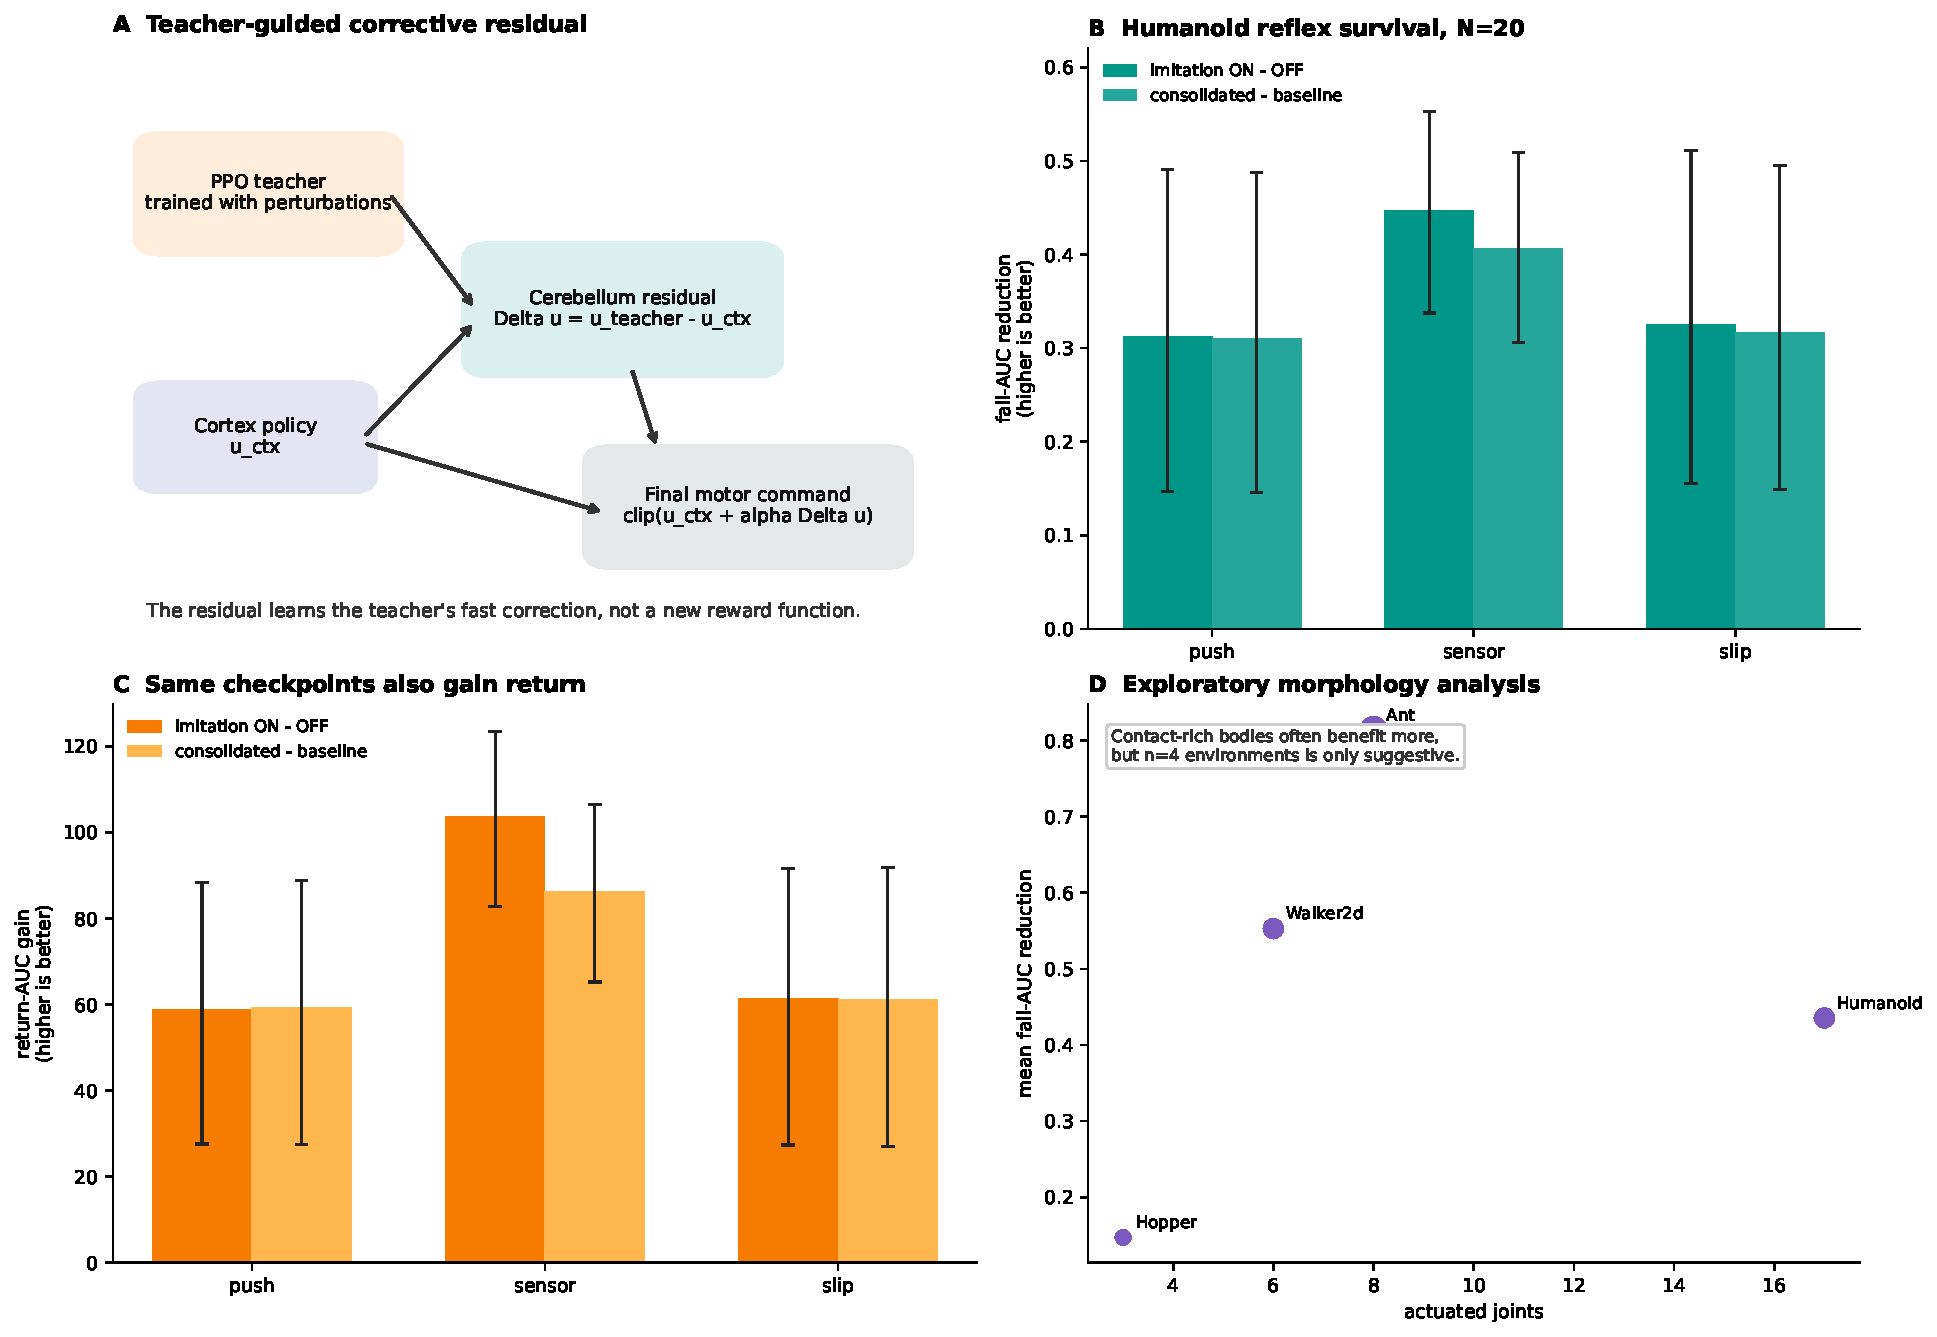
\includegraphics[width=\linewidth]{../Figures/RNNematode-Figures.pdf}
\caption{Main micropublication figure.}
\end{figure}

\section{Negative result: RL-only corrective subcircuits}
The failure ladder matters because it rules out a simple architectural explanation.  The useful ingredient was not the name of the module.  SC-NCAP gain gating, PPO-trained residuals, curriculum residuals, BG-like gates, and stability auxiliary variants did not produce consistent causal robustness improvements.  These results suggest that sparse reward was too indirect for learning a small, fast corrective residual.  Conversely, the successful method should not be presented as a new distillation algorithm; it is a biologically organized use of known supervised residual-learning and distillation ideas \citep{johannink2018residualrl,rusu2015policydistillation,schmitt2018kickstarting}.

The failed variants also differed mechanistically.  In SC-NCAP, prediction error modulated sensory gain before the spinal interface.  In the RL-only residual, a bounded torque correction was available but had to be discovered from sparse return.  In the stability-auxiliary variants, the residual received extra pressure toward uprightness during perturbation windows, but the correction still did not become consistently useful.  These attempts became useful controls: they show that the successful effect is not a generic consequence of adding more modules.

\section{Perturbation sanity}
We also checked that ReflexBench was not only logging intended perturbations.  Table~\ref{tab:sanity} reports simple on/off contrasts from the perturbation sanity runs.  Push values are applied force differences, slip values are the drop in friction scale, and sensor values are clean-versus-corrupted observation differences, each summarized in the native scale of the environment and then reported compactly.  Control episodes had zero event flags.

\begin{table}[h]
\centering
\small
\begin{tabular}{llll}
\toprule
env & push & sensor & slip \\
\midrule
humanoid & 0.588 & 462.616 & 0.607 \\
walker2d & 0.494 & 11.713 & 0.538 \\
ant & 1.098 & 12.697 & 0.645 \\
hopper & 0.100 & 1.664 & 0.410 \\
\bottomrule
\end{tabular}

\caption{Compact perturbation sanity checks.  Nonzero push/slip/sensor contrasts confirm that the perturbations were actually applied.}
\label{tab:sanity}
\end{table}

\section{Teacher quality and safety}
Teacher degradation provided a useful counterfactual.  Students trained from the full teacher improved fall robustness, while students trained from weak teacher checkpoints could become harmful.  In the weak-teacher runs, larger residual corrections tended to predict worse stability outcomes in several windows.  Thus, the residual pathway can inherit useful corrections, but it can also inherit a teacher's mistakes.

\begin{table}[h]
\centering
\small
\begin{tabular}{llrll}
\toprule
teacher\_variant & sweep\_type & n\_seeds & fall\_delta\_ci & return\_delta \\
\midrule
T\_full & push & 3 & -0.261 [-0.385, -0.152] & 54.1 \\
T\_weak & push & 3 & 0.122 [0.000, 0.281] & -20.5 \\
T\_full & sensor & 3 & -0.438 [-0.562, -0.375] & 64.2 \\
T\_weak & sensor & 3 & 0.104 [0.062, 0.125] & -13.1 \\
T\_full & slip & 3 & -0.608 [-1.000, -0.300] & 111.6 \\
T\_weak & slip & 3 & 0.366 [0.000, 0.622] & -37.8 \\
\bottomrule
\end{tabular}

\caption{Teacher-quality replication.  Negative fall deltas are helpful; positive fall deltas are harmful.}
\label{tab:teacher}
\end{table}

This threshold-like pattern helps interpret the result.  If every teacher produced the same student benefit, the result would look like a generic capacity increase.  Instead, the sign of the learned correction depends on teacher competence.  This is consistent with the residual learning a corrective vector field rather than simply smoothing the action.

\section{Structural consolidation}
The consolidation result asks whether the residual is only useful as an extra online module.  We collected trajectories from the residual-ON student and trained a new cortex policy to match the actually executed action.  The consolidation target is:
\[
u_t^{target} = u_t^{final}.
\]
This is stricter than copying the teacher, because $u_t^{final}$ includes the clipped combination of cortex, residual, and optional gate.  In Humanoid, the consolidated cortex-only policy closed most of the baseline-to-imitation fall gap on the default schedule and also generalized under the long-push schedule.  This gives the residual a training role: the correction first appears as a separate pathway, then can be folded back into the main motor command.

\section{Cross-environment and morphology-dependent control demands}
\begin{table}[h]
\centering
\small
\begin{tabular}{lllllr}
\toprule
env & source & metric & mean & sem & n \\
\midrule
Ant-v4 & consolidated\_minus\_baseline & fall & -0.778 & 0.045 & 3 \\
Ant-v4 & consolidated\_minus\_baseline & return & -3.953 & 1.119 & 3 \\
Ant-v4 & imitation\_on\_minus\_off & fall & -0.814 & 0.024 & 3 \\
Ant-v4 & imitation\_on\_minus\_off & return & -4.473 & 1.057 & 3 \\
Hopper-v4 & consolidated\_minus\_baseline & fall & -0.133 & 0.067 & 3 \\
Hopper-v4 & consolidated\_minus\_baseline & return & -15.659 & 0.263 & 3 \\
Hopper-v4 & imitation\_on\_minus\_off & fall & -0.147 & 0.066 & 3 \\
Hopper-v4 & imitation\_on\_minus\_off & return & -15.593 & 0.215 & 3 \\
Walker2d-v4 & consolidated\_minus\_baseline & fall & -0.553 & 0.064 & 3 \\
Walker2d-v4 & consolidated\_minus\_baseline & return & 254.162 & 1.406 & 3 \\
Walker2d-v4 & imitation\_on\_minus\_off & fall & -0.553 & 0.064 & 3 \\
Walker2d-v4 & imitation\_on\_minus\_off & return & 252.326 & 0.995 & 3 \\
Humanoid-v4 & imitation\_on\_minus\_off & fall & -0.361 & 0.080 & 20 \\
Humanoid-v4 & imitation\_on\_minus\_off & return & 74.576 & 14.409 & 20 \\
Humanoid-v4 & consolidated\_minus\_baseline & fall & -0.344 & 0.078 & 20 \\
Humanoid-v4 & consolidated\_minus\_baseline & return & 68.935 & 14.600 & 20 \\
\bottomrule
\end{tabular}

\caption{Cross-environment summary.  Humanoid rows use the N=20 default-schedule result; other environments use the saved cross-environment replication summaries.}
\end{table}

The morphology analysis should be treated cautiously.  Hopper, Walker2d, Ant, and Humanoid are not an evolutionary tree, and four simulated bodies cannot establish a scaling law. The Figure 1D morphology panel uses mean estimates without error bars or confidence regions, so it should be read as a visual summary rather than an inferential regression.  Still, the pattern is useful as a control-demand analysis.  More contact-rich bodies create more transient failure modes; this is exactly where layered corrective control should be useful.  Ant and Humanoid show strong fall reductions.  Hopper is a boundary condition: its underactuated morphology makes conservative corrections able to reduce some falls while hurting return.

\begin{table}[h]
\centering
\small
\begin{tabular}{lrrrll}
\toprule
env & joints & dof & contacts & imit fall delta & cons fall delta \\
\midrule
Hopper-v4 & 3 & 6 & 1 & -0.147 & -0.133 \\
Walker2d-v4 & 6 & 9 & 2 & -0.553 & -0.553 \\
Ant-v4 & 8 & 14 & 4 & -0.814 & -0.778 \\
Humanoid-v4 & 17 & 23 & 2 & -0.435 & -0.295 \\
\bottomrule
\end{tabular}

\caption{Morphology table used for the exploratory scaling plot.  Values may differ from Table~\ref{tab:humanoid} because this plot uses the cross-environment matched summary rather than the full Humanoid N=20 default-schedule summary.  The regression confidence intervals are wide; this table is best read as motivation for future work rather than a final scaling law.}
\label{tab:morphology}
\end{table}

\section{Additional checks}
The report includes the most important controls in the main text: RL-only failures, perturbation sanity checks, teacher-quality degradation, and cross-environment summaries.  The figure below collects these controls in one place so the direction of each check can be inspected visually.

\begin{figure}[h]
\centering
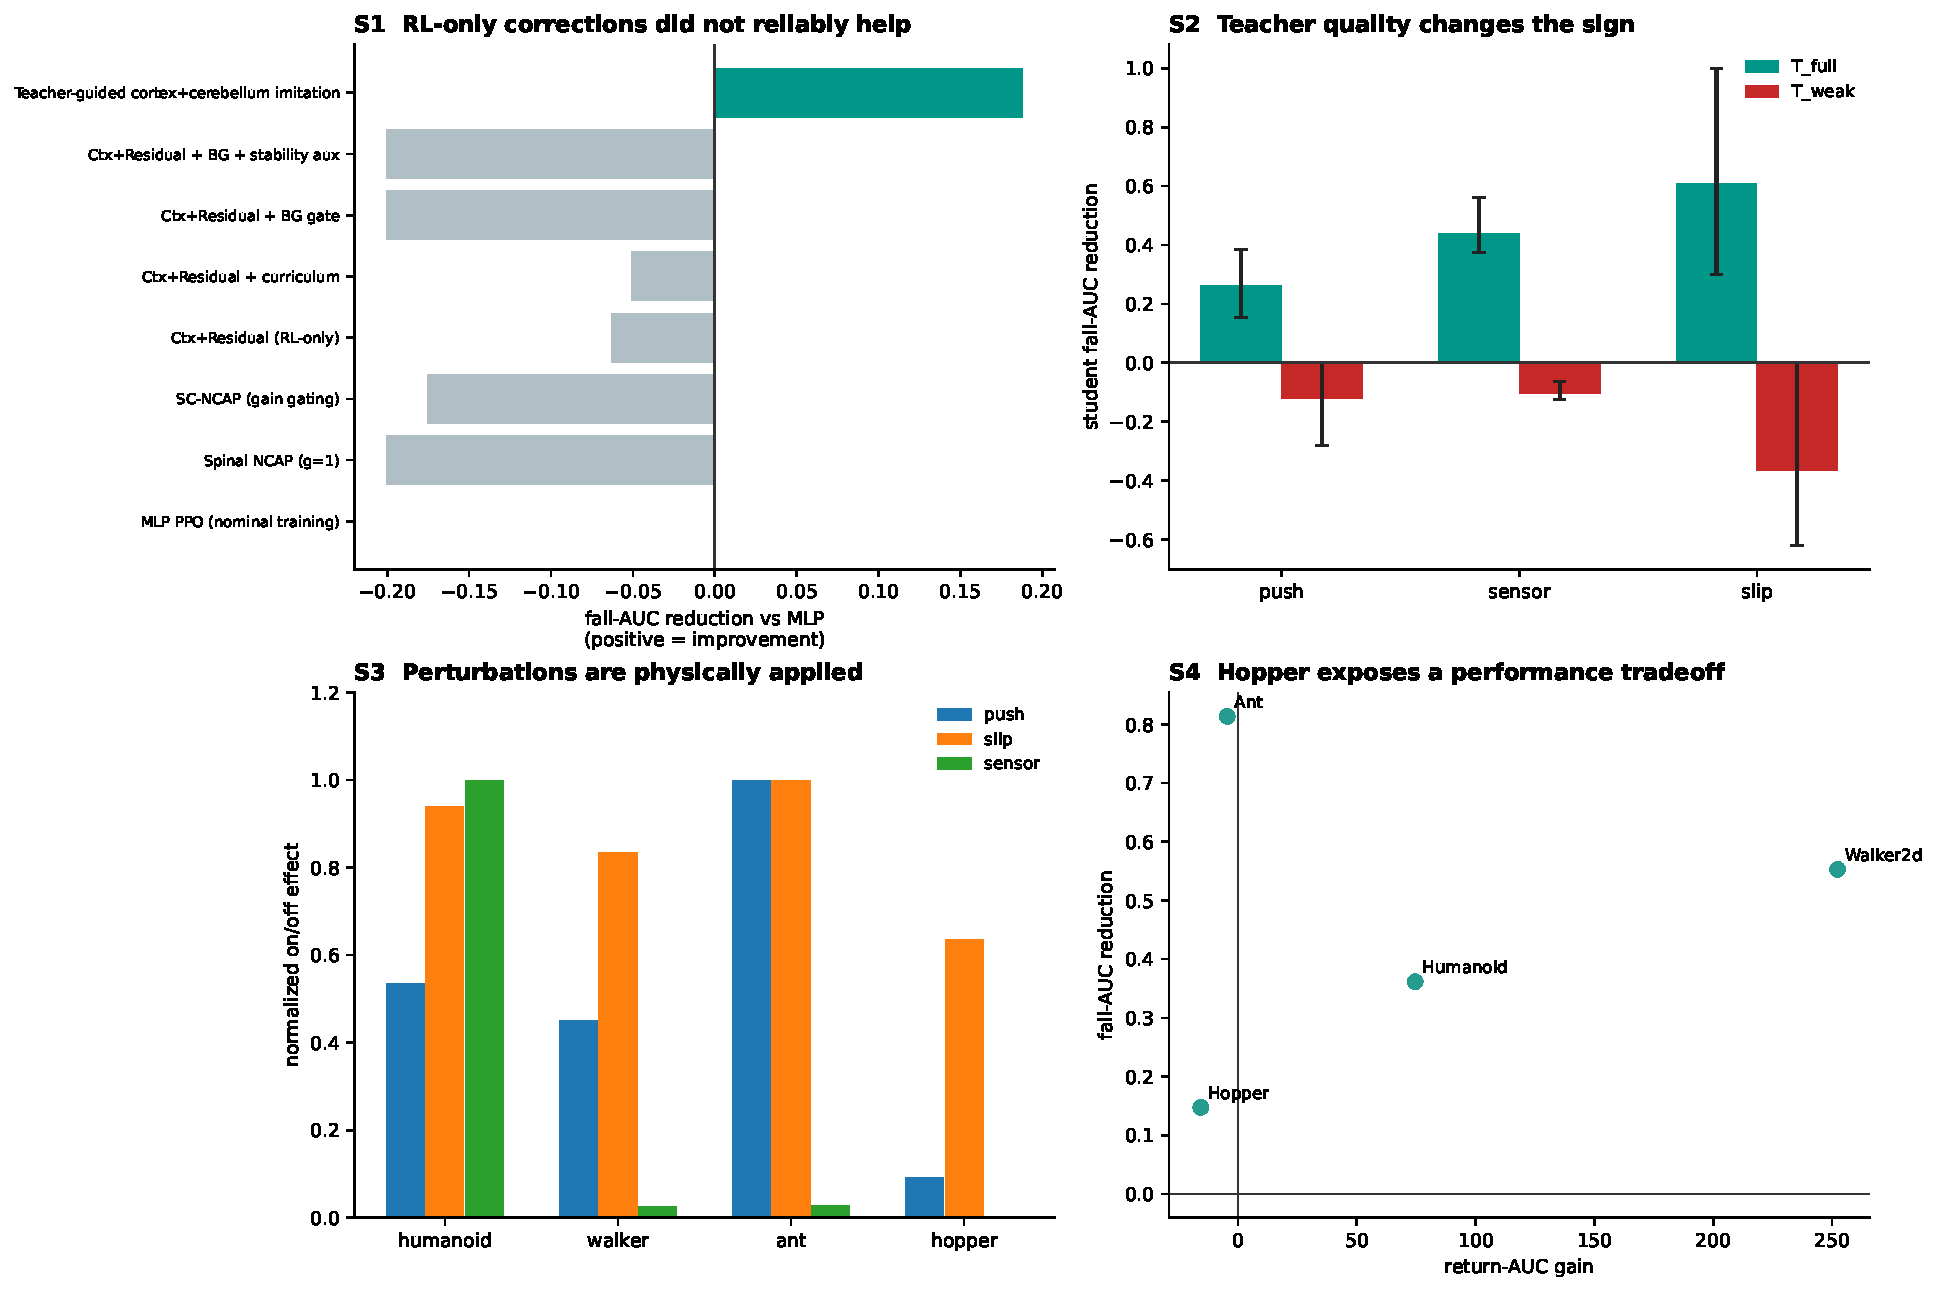
\includegraphics[width=\linewidth]{../Figures/RNNematode-Supplementary-Figures.pdf}
\caption{Supplementary checks: RL-only failure ladder, teacher-quality threshold, perturbation sanity, and cross-environment tradeoffs.  In the failure-ladder panel, positive fall-AUC reduction values indicate improvement over the MLP baseline, while negative values indicate worse fall robustness.}
\end{figure}

\section{Limitations}
This project does not prove that the biological cerebellum implements our exact residual loss.  The better claim is that a cerebellar-inspired supervised correction pathway is a useful engineering abstraction for these locomotion tasks.  Modern privileged-adaptation baselines such as RMA remain important comparators.  Compute fairness is also subtle: the teacher has its own perturbation-trained experience, while the student learns from that experience in supervised form.  We therefore frame the result as a learning-signal result rather than a claim that this architecture dominates all adaptation methods.

\section{Where the code lives}
Core implementation files:
\begin{itemize}
\item \texttt{paper/experiments/sc\_ncap/circuits/cerebellum.py}: bounded residual module.
\item \texttt{paper/experiments/sc\_ncap/policies/cortex\_residual\_policy.py}: cortex plus residual action composition.
\item \texttt{paper/experiments/sc\_ncap/scripts/train\_cerebellum\_imitation.py}: supervised residual imitation.
\item \texttt{paper/experiments/sc\_ncap/scripts/train\_consolidated\_cortex.py}: structural consolidation.
\end{itemize}

\section*{Acknowledgments}
We thank Raymond Chua for senior mentorship, scientific guidance, and feedback on motor-control framing.  We also acknowledge the BrainCAD/NCAP software infrastructure used for circuit templates, MuJoCo wrappers, evaluation, and video export.

\bibliographystyle{plainnat}
\bibliography{../references}
\end{document}
